\documentclass[a4paper]{article}

	%% Language and font encodings
	\usepackage[english,spanish]{babel}
	\usepackage[utf8x]{inputenc}
	\usepackage[T1]{fontenc}
	
	\usepackage{hyperref}
	\usepackage{caption}
	\usepackage{subcaption}
	\usepackage{booktabs}
	
	%% Sets page size and margins
	\usepackage[a4paper,top=3cm,bottom=2cm,left=3cm,right=3cm,marginparwidth=1.75cm]{geometry}
	
	%% Useful packages
	\usepackage{amsmath}
	\usepackage{graphicx}
	\usepackage[colorinlistoftodos]{todonotes}
	\usepackage{float}

	\begin{document}
	
	\title{%
	% \includegraphics[scale = 0.5]{./header_unc.png}\\[1.0 cm]	% University Logo
	  Arquitectura de Computadoras \\
	  \large Ingeniería en Computación FCEFyN - UNC\\
			  Simulador Tomasulo con ROB
	  }
	
	
	  \author{Aguerreberry Matthew. Mat.: 93739112}
	  
	  \maketitle
	  
	  \section{Introducción}
	  
	  Se busca implementar un simulador en Python del algoritmo de Tomasulo con Buffer de reordenamiento.
	  
	  \begin{figure}[H]
	  \centering
	  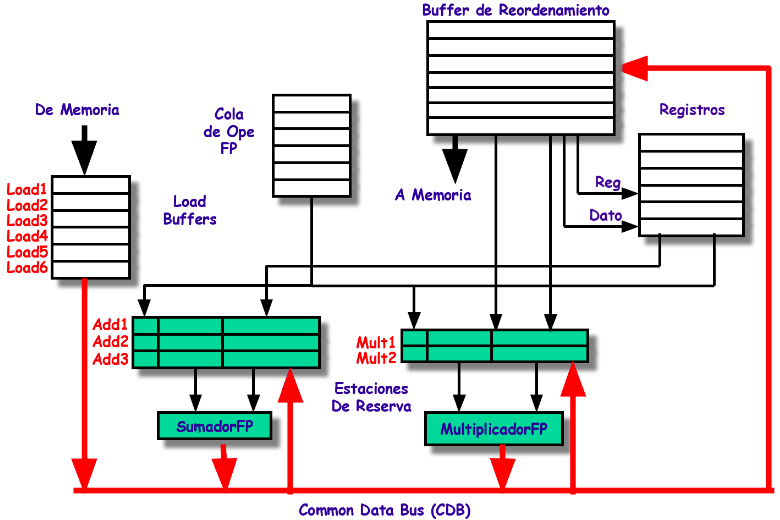
\includegraphics[width=.7\textwidth]{figures/esquema.png}
	  \caption{\label{fig:bloques}Esquema del algoritmo de Tomasulo con ROB}
	  \end{figure}

		
	\subsection{Supuestos}
	
	  Los supuesto a priori y restricciones de la implementación son:

	  \begin{itemize}
		\item La ROB cuenta con 20 entradas.
		\item Propiedades de las unidades funcionales:
		\begin{table}[]
			\centering
			\begin{tabular}{|l|l|l|l|}
				\hline
				\textbf{Unidad de ejecución} & \textbf{Latencia} & \textbf{Intervalo de inicio} & \textbf{Estaciones de Reserva} \\ \hline
				ALU enteros                  & 0                 & 1                            & 2                              \\ \hline
				ALU FP                       & 4                 & 1                            & 3                              \\ \hline
				MULT FP                      & 8                 & 1                            & 2                              \\ \hline
				Accesso a Memoria                      & 4                 & 5                            & 3                              \\ \hline
			\end{tabular}
		\end{table}
	\end{itemize}
		
	\section{Diagramas}

	\subsection*{Estados}

	\begin{figure}[H]
		\centering
		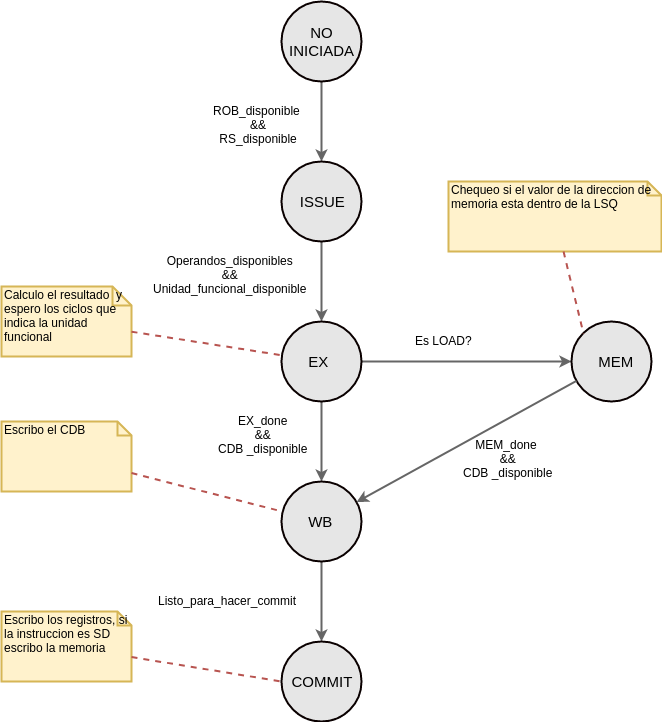
\includegraphics[width=.7\textwidth]{figures/estados.png}
		\caption{\label{fig:estados}Diagrama de estados.}
	\end{figure}
  
	\subsection*{Clases}
	
	\begin{figure}[H]
		\centering
		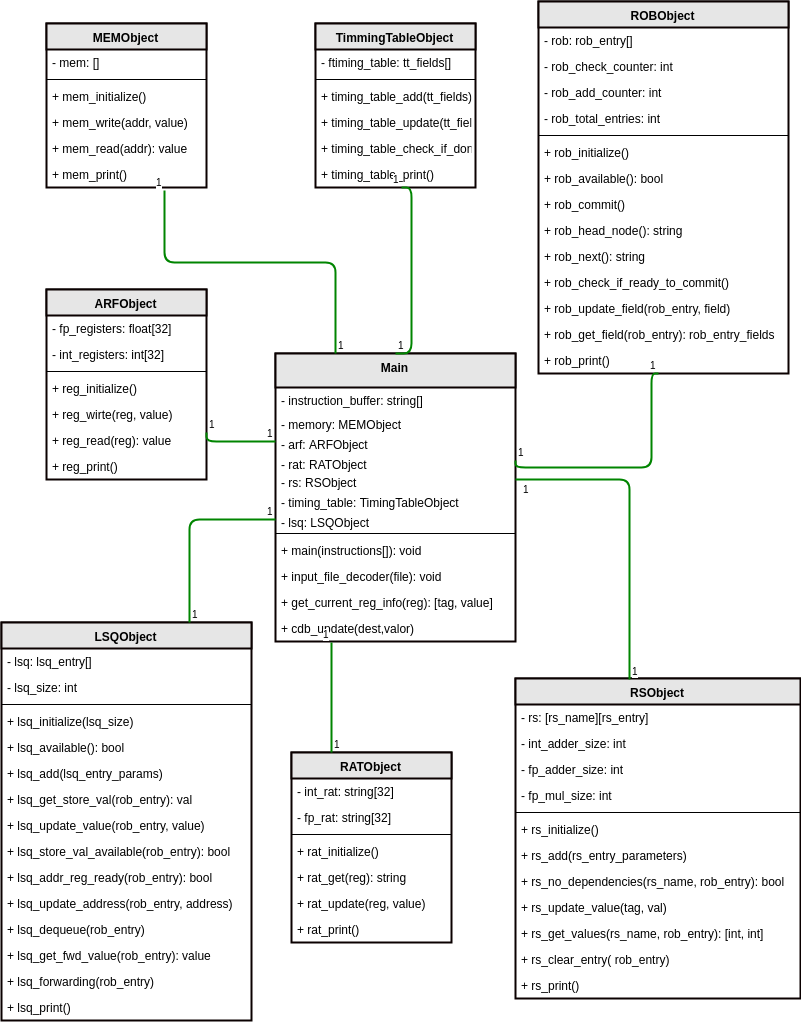
\includegraphics[width=1\textwidth]{figures/clases.png}
		\caption{\label{fig:clases}Diagrama de clases.}
	\end{figure}

	\subsection*{Objetos}

	\begin{figure}[H]		
		\centering
		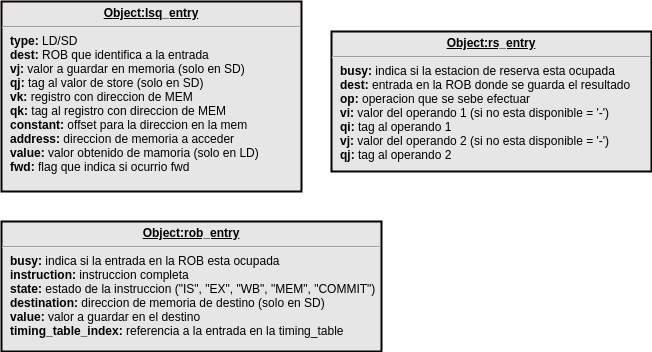
\includegraphics[width=.7\textwidth]{figures/objetos.png}
		\caption{\label{fig:objetos}Diagrama de objetos. Detalle de los campos de las entradas de las respectivas tablas.}
	\end{figure}

	\subsection*{Secuencia}

	\begin{figure}[H]
		\centering
		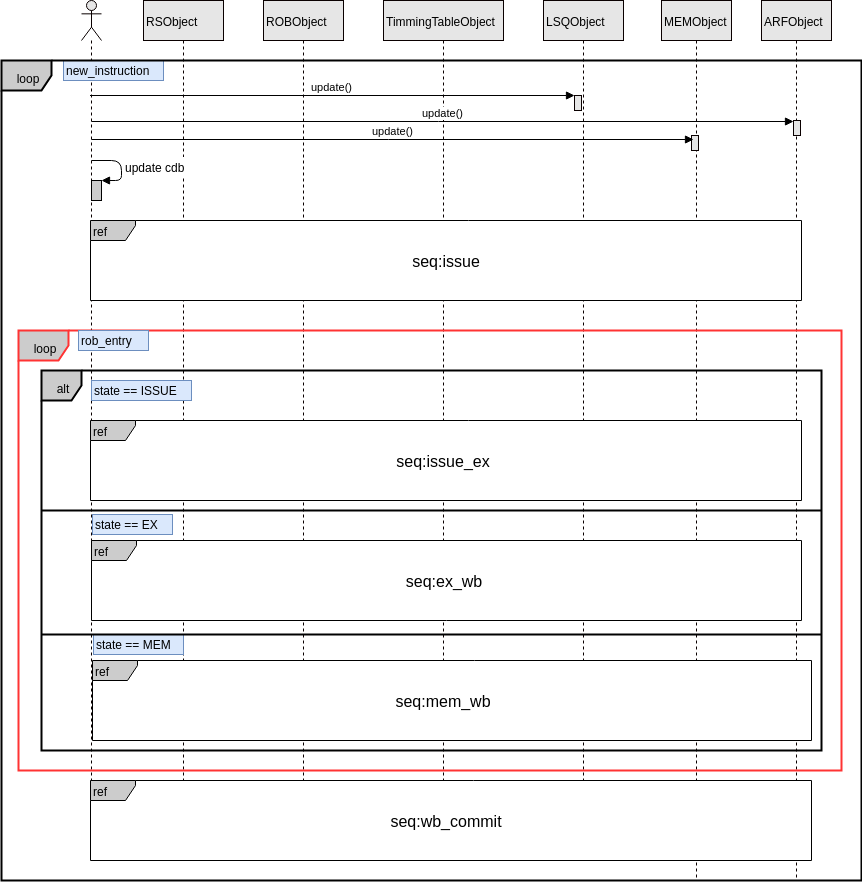
\includegraphics[width=1\textwidth]{figures/main.png}
		\caption{\label{fig:main}Diagrama de secuencia global.}
	\end{figure}

	\begin{figure}[H]
		\centering
		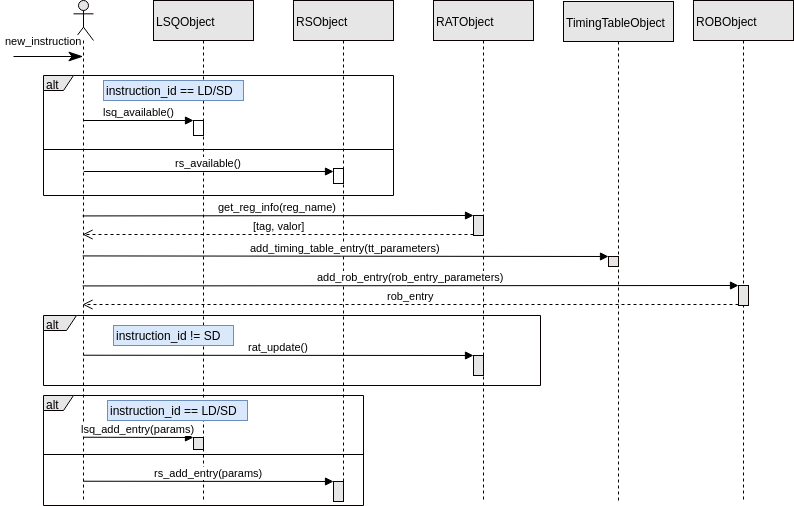
\includegraphics[width=1\textwidth]{figures/sec_issue.png}
		\caption{\label{fig:sec_issue}Diagrama de secuencia. Nueva instrucción.}
	\end{figure}

	\begin{figure}[H]
		\centering
		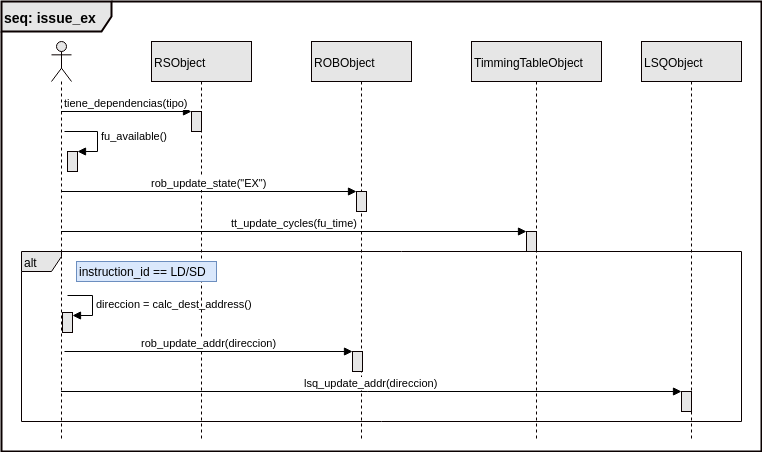
\includegraphics[width=1\textwidth]{figures/issue_ex.png}
		\caption{\label{fig:issue_ex}Diagrama de secuencia. IS a EX.}
	\end{figure}

	\begin{figure}[H]
		\centering
		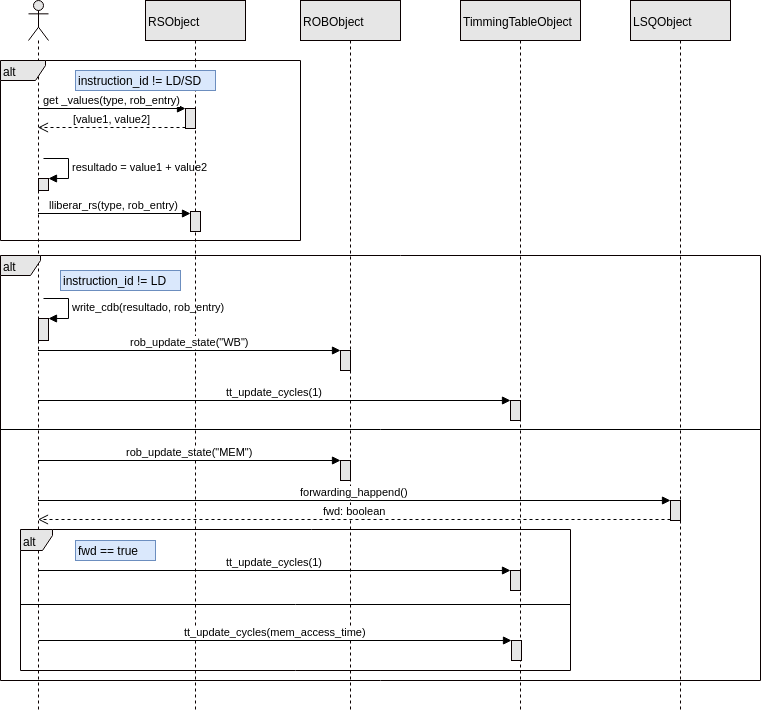
\includegraphics[width=1\textwidth]{figures/ex_wb.png}
		\caption{\label{fig:ex_wb}Diagrama de secuencia. EX a WB.}
	\end{figure}

	\begin{figure}[H]
		\centering
		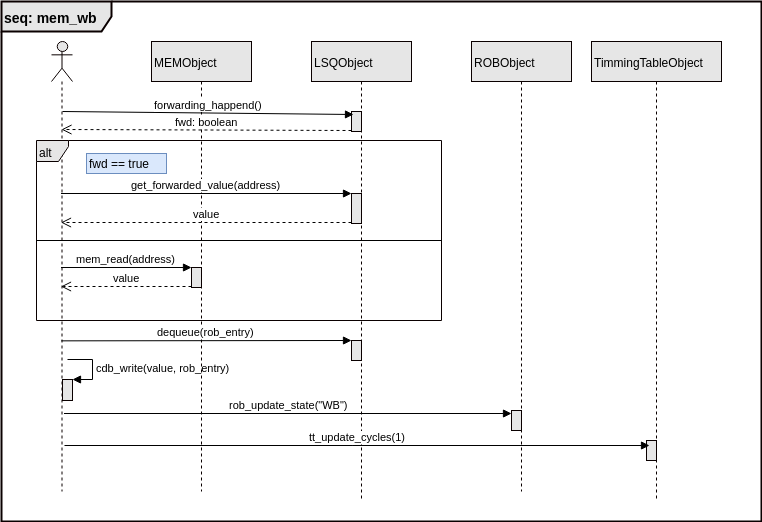
\includegraphics[width=1\textwidth]{figures/mem_wb.png}
		\caption{\label{fig:mem_wb}Diagrama de secuencia. MEM a WB.}
	\end{figure}

	\begin{figure}[H]
		\centering
		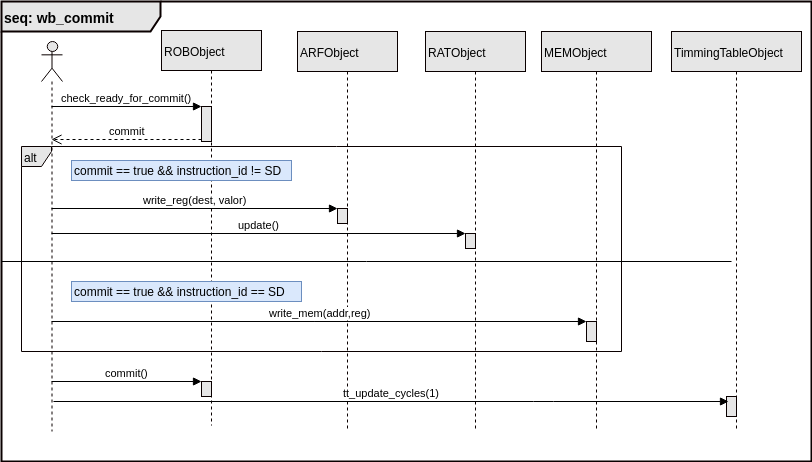
\includegraphics[width=1\textwidth]{figures/wb_commit.png}
		\caption{\label{fig:wb_commit}Diagrama de secuencia. WB a COMMIT.}
	\end{figure}
	
	\section{Verificación y Validación}

	\subsection*{Caso de prueba 1}

	\begin{itemize}
		\item Dependencia de datos entre instrucciones de multiplicación de punto flotante.
		\item Dos instrucciones sin dependencia de datos, que usan la ALU de enteros. 
	\end{itemize}

	\subsubsection*{Procedimiento}

	\textbf{Ejecutar:} python3 tomasulo\_main.py input\_files/input\_file\_1.txt

	\begin{table}[H]
		\centering
		\caption*{Caso 1: Valor inicial de los registros}
		\begin{tabular}{l}
		R1 = 0 \\
		R2 = 3 \\
		R3 = 2 \\
		R4 = 0 \\
		F1 = 0 \\
		F2 = 1.1 \\
		F3 = 2.5 \\
		F4 = 0.0
		\end{tabular}
	\end{table}

	\begin{table}[H]
		\centering
		\caption*{Caso 1: Instrucciones}
		\begin{tabular}{l}
		mult.d F1 F2 F3 \\
		mult.d F4 F1 F2 \\
		add R1 R2 R3 \\
		sub R4 R2 R3
		\end{tabular}
	\end{table}
	
	\subsubsection*{Resultados Esperados}

	\begin{table}[H]
		\centering
		\caption*{Caso 1: Tabla de ciclos}
		\begin{tabular}{|l|l|l|l|l|l|}
		\hline
		\textbf{Inst} & \textbf{IS} & \textbf{EX} & \textbf{MEM} & \textbf{WB} & \textbf{CM} \\ \hline
		0             & 1           & 2           & --           & 10          & 11          \\ \hline
		1             & 2           & 11          & --           & 19          & 20          \\ \hline
		2             & 3           & 4           & --           & 5           & 21          \\ \hline
		3             & 4           & 5           & --           & 6           & 22          \\ \hline
		\end{tabular}
	\end{table}

	\begin{table}[H]
		\centering
		\caption*{Caso 1: Registros y Memoria}
		\begin{tabular}{|l|l|}
		\hline
		\textbf{Nombre / Dirección} & \textbf{Valor} \\ \hline
		F1                          & 2.75           \\ \hline
		F4                          & 3.025          \\ \hline
		R1                          & 5              \\ \hline
		R4                          & 1              \\ \hline
		\end{tabular}
	\end{table}

	\subsubsection*{Resultados del simulador}

	\begin{figure}[H]
	\centering
	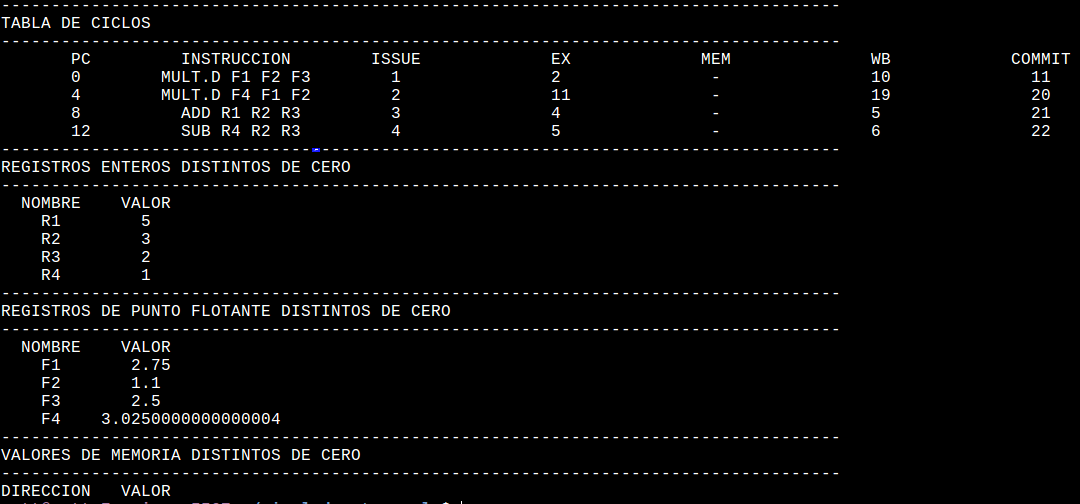
\includegraphics[width=1\textwidth]{figures/test1.png}
	\caption{\label{fig:bloques}Resultados del caso de prueba 1.}
	\end{figure}


	\subsection*{Caso de prueba 2}

	\begin{itemize}
		\item Dependencia estructural en el buffer de load-store. El buffer esta lleno y la próxima instrucción debe esperar que se libere una entrada. 
		\item Riesgo estructural en la etapa de memoria. Cada instrucción de load debe esperar que la anterior finaliza para usar la memoria.
		\item Dependencia de datos en la instrucciones de store. Ambos store deben esperar hasta que finalizan las operaciones de suma.
	\end{itemize}

	\subsubsection*{Procedimiento}

	\textbf{Ejecutar:} python3 tomasulo\_main.py input\_files/input\_file\_2.txt

	\begin{table}[H]
		\centering
		\caption*{Caso 2: Valor inicial de la memoria}
		\begin{tabular}{l}
			0x4 = 3.3 \\
			0x8 = 2.2 \\
			0xc = 3.4 \\
			0x10 = 5.5			
		\end{tabular}
	\end{table}

	\begin{table}[H]
		\centering
		\caption*{Caso 2: Instrucciones}
		\begin{tabular}{l}
			ld F1 1(R0) \\
			ld F2 2(R0) \\
			ld F3 3(R0) \\
			ld F4 4(R0) \\
			add.d F5 F1 F2 \\
			add.d F6 F5 F3 \\
			Sd F5 20(R0) \\
			Sd F6 24(R0)
		\end{tabular}
	\end{table}

	\subsubsection*{Resultados Esperados}

	\begin{table}[H]
		\centering
		\caption*{Caso 2: Tabla de ciclos}
		\begin{tabular}{|l|l|l|l|l|l|}
			\hline
			\textbf{Inst} & \textbf{IS} & \textbf{EX} & \textbf{MEM} & \textbf{WB} & \textbf{CM} \\ \hline
			0             & 1           & 2           & 3            & 7           & 8           \\ \hline
			1             & 2           & 3           & 7            & 11          & 12          \\ \hline
			2             & 3           & 4           & 11           & 15          & 16          \\ \hline
			3             & 8           & 9           & 15           & 19          & 20          \\ \hline
			4             & 9           & 12          & --           & 16          & 21          \\ \hline
			5             & 10          & 17          & --           & 21          & 22          \\ \hline
			6             & 12          & 13          & --           & 17          & 23          \\ \hline
			7             & 16          & 17          & --           & 22          & 27          \\ \hline
			\end{tabular}
	\end{table}

	\begin{table}[H]
		\centering
		\caption*{Caso 2: Registros y Memoria}
		\begin{tabular}{|l|l|}
			\hline
			\textbf{Nombre / Dirección} & \textbf{Valor} \\ \hline
			F1                          & 3.3            \\ \hline
			F2                          & 2.2            \\ \hline
			F3                          & 3.4            \\ \hline
			F4                          & 5.5            \\ \hline
			F5                          & 5.5            \\ \hline
			F6                          & 8.9            \\ \hline
			0x50                        & 5.5            \\ \hline
			0x60                        & 8.9            \\ \hline
		\end{tabular}
	\end{table}

	\subsubsection*{Resultados del simulador}

	\begin{figure}[H]
	\centering
	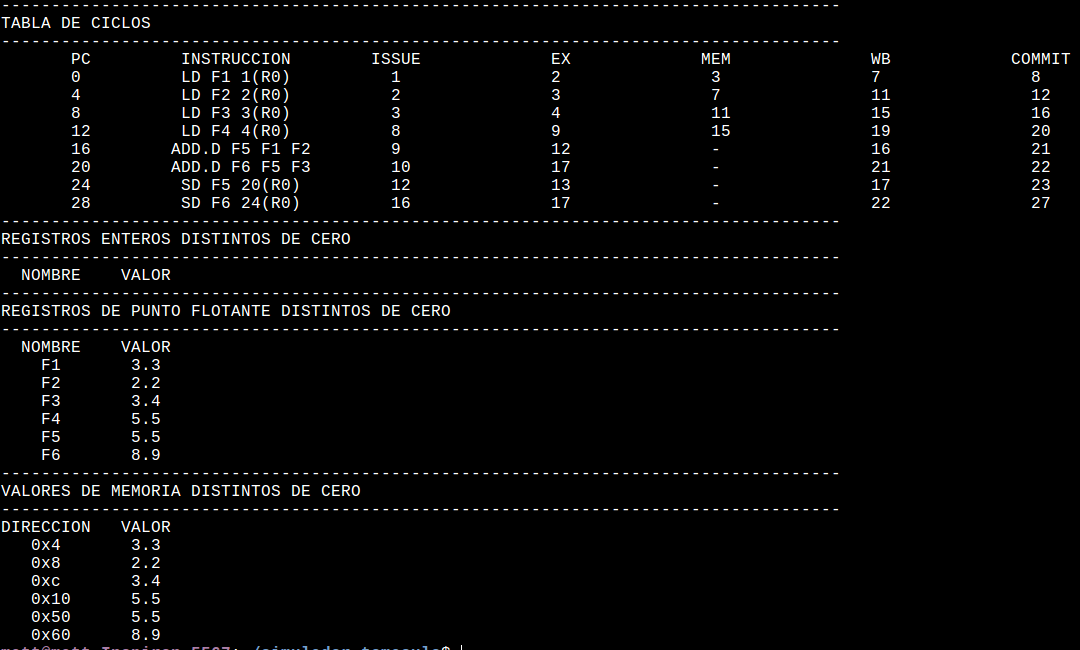
\includegraphics[width=1\textwidth]{figures/test2.png}
	\caption{\label{fig:bloques}Resultados del caso de prueba 2.}
	\end{figure}


	\subsection*{Caso de prueba 3}

	\begin{itemize}
		\item Este test muestra el \textit{forwarding} entre las operaciones de load y store en el buffer de load-store.
	\end{itemize}

	\subsubsection*{Procedimiento}

	\textbf{Ejecutar:} python3 tomasulo\_main.py input\_files/input\_file\_3.txt

	\begin{table}[H]
		\centering
		\caption*{Caso 3: Valor inicial de los registros y memoria}
		\begin{tabular}{l}
			F1 = 7.8 \\
			F2 = 0 \\
			F3 = 0 \\
			0x4 = 3 \\
			0x8 = 2 \\
			0xc = 3.4 \\
			0x10 = 5.5
		\end{tabular}
	\end{table}

	\begin{table}[H]
		\centering
		\caption*{Caso 3: Instrucciones}
		\begin{tabular}{l}
			Sd F1 1(R0) \\
			Ld F2 1(R0) \\
			Ld F3 1(R0) \\
			Ld F4 1(R0)
		\end{tabular}
	\end{table}

	\subsubsection*{Resultados Esperados}

	\begin{table}[H]
		\centering
		\caption*{Caso 3: Tabla de ciclos}
		\begin{tabular}{|l|l|l|l|l|l|}
			\hline
			\textbf{Inst} & \textbf{IS} & \textbf{EX} & \textbf{MEM} & \textbf{WB} & \textbf{CM} \\ \hline
			0             & 1           & 2           & --           & 3           & 4           \\ \hline
			1             & 2           & 3           & 4            & 5           & 6           \\ \hline
			2             & 3           & 4           & 5            & 6           & 7           \\ \hline
			3             & 8           & 9           & 10           & 14          & 15          \\ \hline
			\end{tabular}
	\end{table}

	\begin{table}[H]
		\centering
		\caption*{Caso 3: Registros y Memoria}
		\begin{tabular}{|l|l|}
			\hline
			\textbf{Nombre / Dirección} & \textbf{Valor} \\ \hline
			F2                          & 7.8            \\ \hline
			F3                          & 7.8            \\ \hline
			F4                          & 7.8            \\ \hline
			0x4                         & 7.8            \\ \hline
		\end{tabular}
	\end{table}

	\subsubsection*{Resultados del simulador}

	\begin{figure}[H]
	\centering
	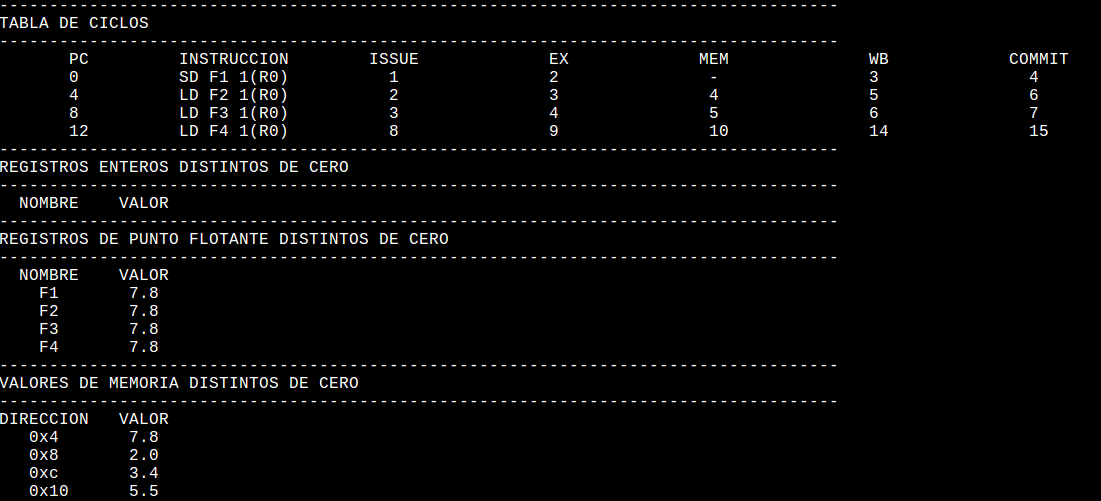
\includegraphics[width=1\textwidth]{figures/test3.png}
	\caption{\label{fig:bloques}Resultados del caso de prueba 3.}
	\end{figure}


	\subsection*{Caso de prueba 4}

	\begin{itemize}
		\item Los operandos de la instrucción store, ambos depende de resutlados de operaciones anteriores, la suma flotante y la suma de enteros. 
	\end{itemize}

	\subsubsection*{Procedimiento}

	\textbf{Ejecutar:} python3 tomasulo\_main.py input\_files/input\_file\_4.txt

	\begin{table}[H]
		\centering
		\caption*{Caso 4: Valor inicial de los registros y memoria}
		\begin{tabular}{l}
			R1 = 0 \\
			R2 = 2 \\
			F1 = 0  \\
			F2 = 1.1 \\
			F3 = 2.5 \\
			F4 = 0.0 \\
			F5 = 1.5 \\
			0x4 = 3 \\
			0x8 = 2 \\
			0xc = 3.4 \\
		\end{tabular}
	\end{table}

	\begin{table}[H]
		\centering
		\caption*{Caso 4: Instrucciones}
		\begin{tabular}{l}
			mult.d F1 F2 F3 \\
			add.d F4 F2 F5 \\
			Addi R1 R1 1 \\
			Sd F4 8(R1)
		\end{tabular}
	\end{table}

	\subsubsection*{Resultados Esperados}

	\begin{table}[H]
		\centering
		\caption*{Caso 4: Tabla de ciclos}
		\begin{tabular}{|l|l|l|l|l|l|}
			\hline
			\textbf{Inst} & \textbf{IS} & \textbf{EX} & \textbf{MEM} & \textbf{WB} & \textbf{CM} \\ \hline
			0             & 1           & 2           & --           & 10          & 11          \\ \hline
			1             & 2           & 3           & --           & 7           & 12          \\ \hline
			2             & 3           & 4           & --           & 5           & 13          \\ \hline
			3             & 4           & 6           & --           & 8           & 14          \\ \hline
			\end{tabular}
	\end{table}

	\begin{table}[H]
		\centering
		\caption*{Caso 4: Registros y Memoria}
		\begin{tabular}{|l|l|}
			\hline
			\textbf{Nombre / Dirección} & \textbf{Valor} \\ \hline
			F2                          & 7.8            \\ \hline
			F3                          & 7.8            \\ \hline
			F4                          & 7.8            \\ \hline
			0x4                         & 7.8            \\ \hline
		\end{tabular}
	\end{table}

	\subsubsection*{Resultados del simulador}

	\begin{figure}[H]
	\centering
	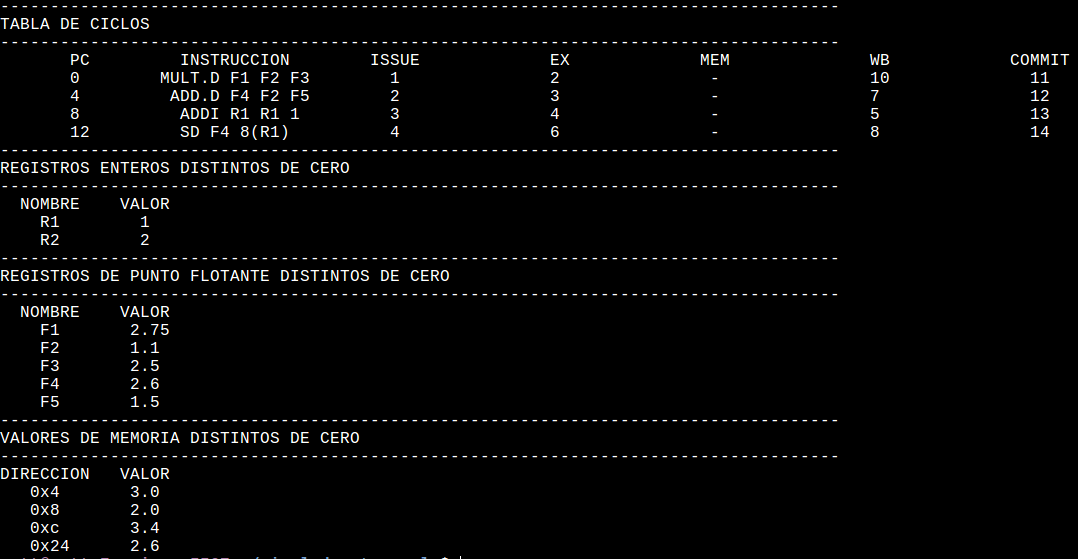
\includegraphics[width=1\textwidth]{figures/test4.png}
	\caption{\label{fig:bloques}Resultados del caso de prueba 4.}
	\end{figure}


	\subsection*{Caso de prueba 5}

	\begin{itemize}
		\item Dependencia estructural en la estación de reserva de las multiplicaciones flotantes. La instrucción libera la estación de reserva cuando pasa a writeback.  
	\end{itemize}

	\subsubsection*{Procedimiento}

	\textbf{Ejecutar:} python3 tomasulo\_main.py input\_files/input\_file\_5.txt

	\begin{table}[H]
		\centering
		\caption*{Caso 5: Valor inicial de los registros}
		\begin{tabular}{l}
			F1 = 0 \\
			F2 = 1.1 \\
			F3 = 2.5 \\
			F4 = 0.0 \\
			F5 = 1.5 \\
			F6 = 1.5 \\
			F7 = 0 \\
			F8 = 3.5 \\
			F9 = 3.5 \\
			F10 = 0 \\
			F11 = 5.5 \\
			F12 = 5.5
		\end{tabular}
	\end{table}

	\begin{table}[H]
		\centering
		\caption*{Caso 5: Instrucciones}
		\begin{tabular}{l}
			mult.d F1 F2 F3 \\
			mult.d F4 F5 F6 \\
			mult.d F7 F8 F9 \\
			mult.d F10 F11 F12
		\end{tabular}
	\end{table}

	\subsubsection*{Resultados Esperados}

	\begin{table}[H]
		\centering
		\caption*{Caso 5: Tabla de ciclos}
		\begin{tabular}{|l|l|l|l|l|l|}
			\hline
			\textbf{Inst} & \textbf{IS} & \textbf{EX} & \textbf{MEM} & \textbf{WB} & \textbf{CM} \\ \hline
			0             & 1           & 2           & --           & 10          & 11          \\ \hline
			1             & 2           & 3           & --           & 11          & 12          \\ \hline
			2             & 11          & 12          & --           & 20          & 21          \\ \hline
			3             & 12          & 13          & --           & 21          & 22          \\ \hline
			\end{tabular}
	\end{table}

	\begin{table}[H]
		\centering
		\caption*{Caso 5: Registros y Memoria}
		\begin{tabular}{|l|l|}
			\hline
			\textbf{Nombre / Dirección} & \textbf{Valor} \\ \hline
			F1                          & 2.75           \\ \hline
			F4                          & 2.25           \\ \hline
			F7                          & 12.25          \\ \hline
			F10                         & 30.25          \\ \hline
		\end{tabular}
	\end{table}

	\subsubsection*{Resultados del simulador}

\begin{figure}[H]
	\centering
	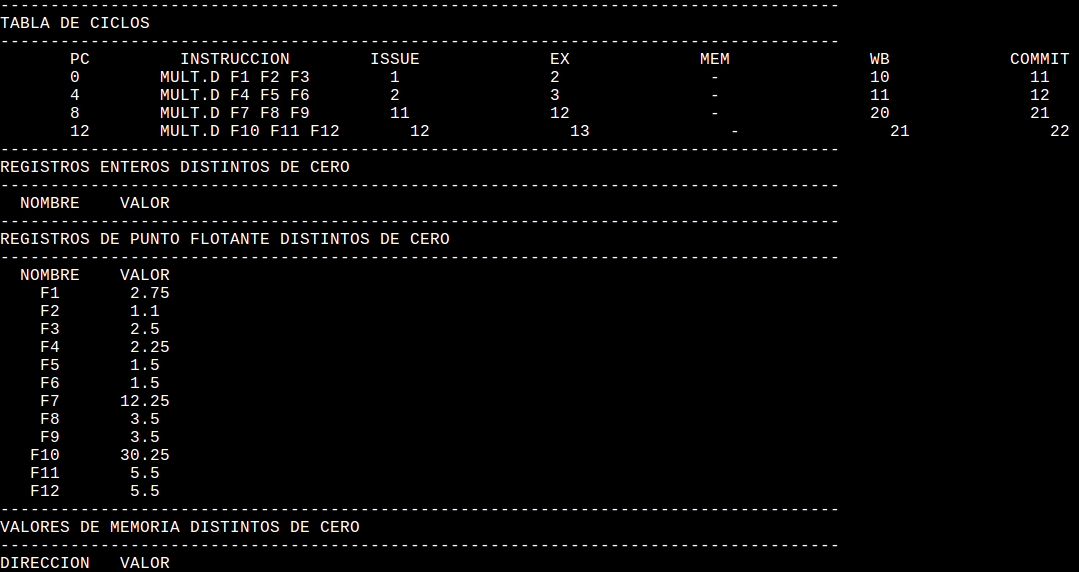
\includegraphics[width=1\textwidth]{figures/test5.png}
	\caption{\label{fig:bloques}Resultados del caso de prueba 5.}
	\end{figure}


	\section{Conclusiones}
	
	Para que un procesador pueda aumentar su \textit{throughput} debe ejecutar las instrucciones fuera de orden. Sin embargo, esto trae complicaciones ya que surgen riesgos de datos, excepciones imprecisas, riesgos a través de la memoria y problemas cuando se mal predice un salto.
	
	El algoritmo de Tomasulo evita los riesgos de datos empleando la técnica de renombramiento de registros. A su vez, para solventar el problema de excepciones imprecisas y recuperación de saltos mal predichos, se emplea el buffer de reordenamiento que asegura que las instrucciones finalizan en orden y así poder recuperar el estado del procesador.	Asimismo, los riegos de memoria se solucionan utilizando un buffer dedicado a las operaciones de load y store que asegura que estas se ejecuten sin conflictos. 

	Es por esto que los procesadores de hoy en día poseen una implementación análoga a este algoritmo en su arquitectura. 

	\end{document}